\chapter{Fundamentação Teórica}
\label{cap:fundamentacao-teorica}
\phantom{0}

Neste capítulo são detalhados os tópicos necessários para compreensão das técnicas usadas na elaboração do método proposto. As seções a seguir abordam conceitos sobre o exame de TC, o rim e tumores renais, aprendizado profundo e as métricas de desempenho para validar os resultados experimentais.

\section{Rins e Tumores Renais}
\label{sec:rins-e-tumores-renais}

Os rins são órgãos bilaterais em forma de feijão, de cor marrom-avermelhada e localizados na região posterior do abdômen. Geralmente, o rim direito é ligeiramente menor e mais baixo que o esquerdo devido à presença do fígado. Cada rim pesa cerca de 125-170 gramas nos homens e 115-155 gramas nas mulheres, e são revestidos por uma cápsula renal fibrosa e resistente. Além disso, duas camadas de gordura servem como proteção \cite{tim_newman}.

Internamente, os rins têm uma estrutura intrincada e única, conforme ilustrado na Figura~\ref{fig:anatomia-rins-interno}. O rim apresenta uma camada central com uma cor mais escura (medula) e uma camada periférica mais clara (córtex). Na medula renal, encontram-se as pirâmides renais, estruturas que têm o formato de um cone. O ápice de uma pirâmide renal está voltado para o córtex, e termina em uma papila que se despeja no cálice menor. O córtex se estende da cápsula até a base das pirâmides renais e também se encontra entre essas estruturas, formando as colunas renais~\cite{oliver_jones,vanessa_sardinha}.

O córtex e a medula recebem sangue pela artéria renal e são drenados pela veia renal. Há também uma estrutura achatada e com formato de funil (pelve renal), responsável pela coleta da urina. A pelve se ramifica em direção à medula, formando cálices maiores e menores. Por fim, em cada rim, a margem medial é marcada por uma fissura profunda, conhecida como hilo renal. O hilo renal atua como uma porta de entrada para o rim, onde normalmente os vasos renais e o ureter entram e saem do rim~\cite{oliver_jones,vanessa_sardinha,tim_newman}.

\begin{figure}[!ht]
    \centering
    \caption{Estrutura interna do rim.}
    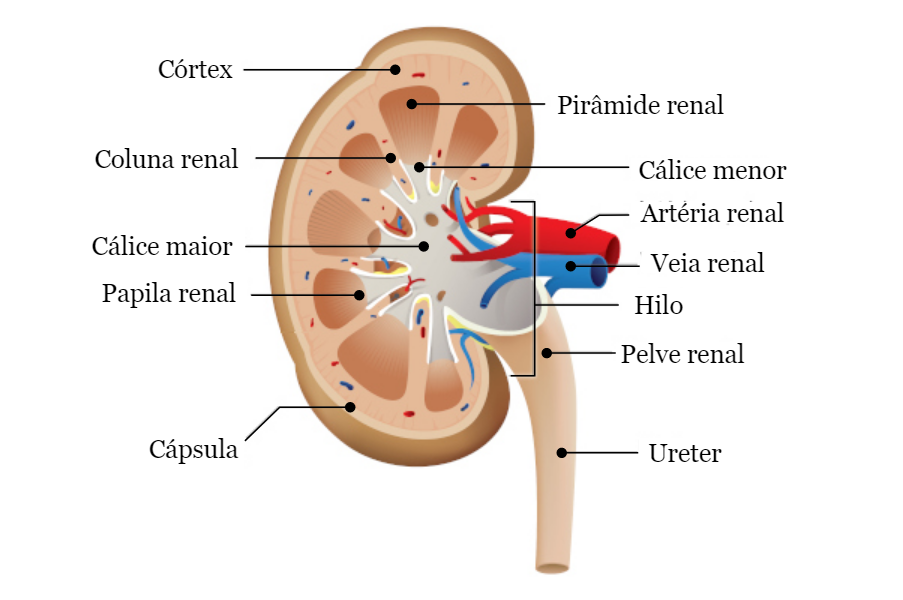
\includegraphics[width=0.85\textwidth]{figuras/anatomia-rins-interno.png}
    \legend{Fonte: \cite{vanessa_sardinha}.}
    \label{fig:anatomia-rins-interno}
\end{figure}

O principal papel dos rins é manter a homeostase. Isso significa que os rins gerenciam os níveis de fluidos, o equilíbrio eletrolítico e outros fatores que mantêm o ambiente interno do corpo consistente e confortável. Além disso, desempenham um amplo espectro de funções, tais como: remover uma série de resíduos a serem eliminados pela urina, reabsorção de nutrientes do sangue, manter o pH estável e regular a osmolaridade e a pressão arterial \cite{american_cancer,tim_newman,world_cancer}.

%Os rins são circuncidados em camadas externas complexas de fáscia e gordura, organizados da seguinte forma (profundo para superficial): cápsula renal, que é cápsula fibrosa resistente intimamente colada à superfície do órgão; gordura perirrenal, trata-se de uma coleção de gordura extraperitoneal; fáscia renal, responsável por envolver os rins e as glândulas supra-renais; e a gordura pararrenal, localizada principalmente na face póstero-lateral do rim~\cite{oliver_jones}. A Figura~\ref{fig:anatomia-rins-externo} ilustra as camadas externas do rim.

% \begin{figure}[!ht]
%     \centering
%     \caption{As camadas externas do rim.}
%     \includegraphics[width=0.8\textwidth]{figuras/anatomia-rins-externo2.png}
%     \legend{Fonte: Adaptado de \cite{oliver_jones}.}
%     \label{fig:anatomia-rins-externo}
% \end{figure}

Uma série de doenças pode afetar os rins, tais como: nefropatia diabética, insuficiência renal, hidronefrose renal, síndrome nefrótica, pedras nos rins e nefrite intersticial. Além disso, quando as células renais começam a se multiplicar de forma acelerada, podem surgir tumores renais. Os tumores renais podem ser benignos ou malignos. Os benignos não se espalham nem atacam os tecidos, mas os malignos podem ser agressivos a ponto de atingir outros órgãos por meio da corrente sanguínea. O câncer renal maligno mais comum é o carcinoma de células renais~\cite{SHUCH201585,tim_newman}.

A maioria dos casos de câncer renal tem cura com um diagnóstico precoce. Para iniciar o tratamento adequado do câncer renal, a segmentação acurada dos rins é necessária. Portanto, as informações estruturais do rim são analisadas por meio de exames de ultrassom, Ressonância Magnética (RM) ou TC de abdômen. Embora as imagens RM tenham sido usadas para segmentação renal em alguns estudos na literatura~\cite{goceri2011automatic,7424483}, a TC, dentre as modalidades disponíveis, é considerada o padrão ouro, especialmente para o diagnóstico de câncer precoce~\cite{kaur2016survey}. Além disso, a TC é muito útil no estadiamento (verificação da extensão para outros órgãos) e no planejamento terapêutico.

\section{Tomografia Computadorizada}
\label{sec:tumografia-computadorizada}

Para planejar o tratamento radioterápico, é necessário obter informações sobre os tumores renais, como tamanho e a localização exata. Para isso, é necessária uma imagem tridimensional detalhada da região do abdômen do paciente, geralmente realizada por meio do exame de TC. Essas informações são eventualmente usadas para orientar o radioterapeuta a produzir o melhor tratamento radioterápico para cada paciente.

A TC é um exame não invasivo, indolor e rápido, que combina uma série de imagens de raios-X obtidas de diferentes ângulos do corpo do paciente, produzindo sinais que são processados pelo computador para gerar imagens transversais (fatias) dos ossos, vasos sanguíneos e tecidos moles~\cite{Buzug2011}. Portanto, a TC funciona como outros exames de raios-X, mas fornece imagens mais detalhadas devido à emissão de vários feixes de raios-X ao mesmo tempo~\cite{gwynne2012image}.

Os feixes de raios-X são emitidos por uma fonte e coletados por um conjunto de detectores que permitem avaliar a quantidade de radiação que é absorvida pelos diferentes tecidos. Os detectores são posicionados no lado diametralmente oposto para captar os feixes que passam pelos objetos observados. Finalmente, os dados coletados pelos detectores são processados e digitalizados em \textit{pixels} que apresentam uma escala de cinza relacionada à atenuação sofrida pelos raios-X (medida da facilidade com que um material pode ser penetrado por um feixe de energia), expressa por uma escala numérica expressa em unidades Hounsfield (\textit{Hounsfield Units} - HU)~\cite{Buzug2011}. A HU é calculada com base em uma transformação linear do coeficiente de atenuação linear da linha de base do feixe de raios X~\cite{ADAMS2012277}.

Para a realização do exame, o paciente é posicionado no tomógrafo e imobilizado com suportes e fitas de fixação. O tomógrafo é uma máquina com um túnel no centro onde, durante o exame, o paciente fica deitado sobre uma mesa estreita que desliza dentro do túnel. Cortes axiais são feitos para verificar o posicionamento e alinhamento do paciente tomando como referência o isocentro (ponto onde os feixes de radiação se cruzam). Em seguida, são realizadas radiografias digitais (topograma), que programam as sequências de imagens (fatias) e a espessura dos cortes~\cite{Buzug2011,gwynne2012image}. A Figura~\ref{fig:equipamentoCT} ilustra um exemplo de equipamento de TC.

\begin{figure}[!ht]
    \centering
    \caption{Equipamento de TC.}
    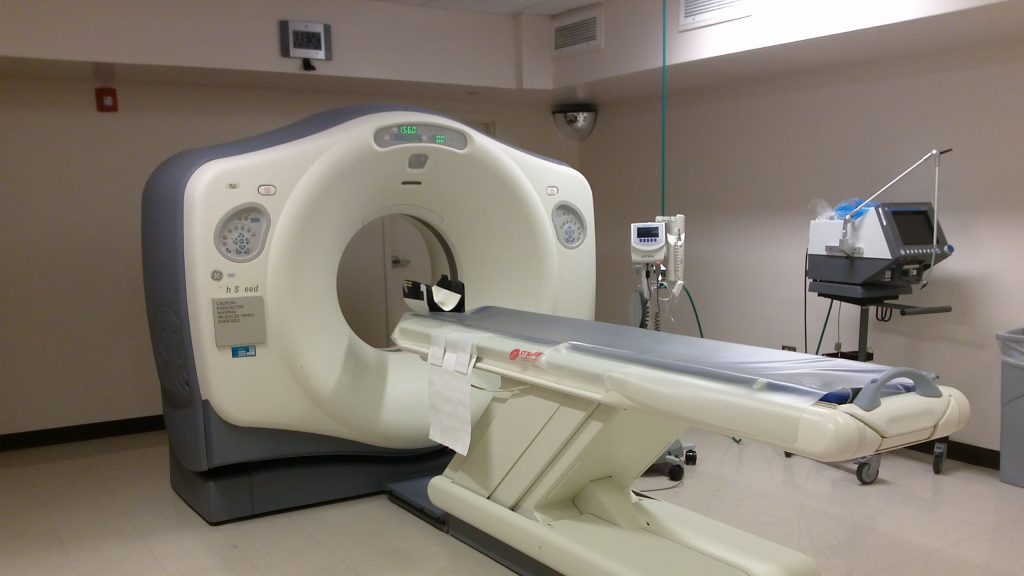
\includegraphics[width=0.9\textwidth]{figuras/equipamento-CT.jpg}
    \legend{Fonte: \cite{equipamento_CT}.}
    \label{fig:equipamentoCT}
\end{figure}

Uma vez que várias fatias sucessivas são coletadas pelo computador da máquina, elas são “empilhadas” digitalmente para formar uma imagem tridimensional do paciente que permite a identificação e localização mais fácil das estruturas básicas do corpo, bem como possíveis tumores ou anormalidades. Para melhorar a interpretação dos resultados e garantir diagnósticos mais precisos, a administração de contraste intravenoso pode ser solicitada antes da aquisição das imagens. Estas substâncias são usadas para aumentar a visibilidade e a diferenciação entre tumores e estruturas circundantes normais. O produto para se obter esse contraste é geralmente administrado por via oral (engolido) ou por via intravenosa (injetado). Após a obtenção das imagens, o contraste é eliminado pela urina.

\section{Processamento Digital de Imagens}
\label{sec:processamento-digital-imagens}

O processamento digital de imagens é definido como um conjunto de técnicas computacionais que transformam uma imagem de entrada em uma saída desejada~\cite{gonzalez2008digital}. Esse conjunto de técnicas permite extrair e identificar informações de imagens e melhorar a qualidade visual de aspectos estruturais, facilitando a percepção humana e a interpretação automática por meio de máquinas~\cite{pedrini2008analise}.

Existem vários algoritmos com propósitos muito específicos, que juntos formam a metodologia final. Portanto, uma metodologia difere de outra na forma como compõe suas etapas ou ferramentas, mas normalmente segue as etapas apresentadas por \citeonline{gonzalez2008digital}:

\begin{enumerate}
    \item Aquisição das imagens: as imagens são capturadas por meio de um dispositivo ou sensor e transformadas em um formato que pode ser processado posteriormente. Porém, como resultado desse processo, a imagem resultante pode apresentar falhas devido às condições de iluminação ou às características do dispositivo, por exemplo;
    
    \item Pré-processamento: o objetivo é melhorar a qualidade da imagem por meio de técnicas para reduzir o ruído, realçar o contraste e suavizar certas estruturas da imagem;
    
    \item Segmentação: consiste em localizar e extrair áreas de interesse contidas na imagem, com o objetivo de dividir a imagem isolando os diferentes objetos que a compõem;
    
    \item Representação e descrição: denominada de extração de características, pois extrai informações que podem ser usadas para discriminar classes de objetos;
    
    \item Reconhecimento e interpretação: reconhecimento é o processo que atribui um identificador aos objetos da imagem. A interpretação consiste em atribuir um significado ao conjunto de objetos reconhecidos.
\end{enumerate}

A saída de uma etapa é usada como entrada para a próxima etapa, sendo que cada entrada e saída pode ser ou não uma imagem digital. Uma metodologia de processamento de imagem pode conter apenas um subconjunto de todas as etapas apresentadas~\cite{BRAZ:2014}.

\section{Especificação do Histograma}
\label{sec:especificacao-histograma}

O histograma básico de uma imagem digital é uma função que gera a distribuição dos valores de intensidade presentes em uma imagem, com níveis de intensidade variando no intervalo de $\left[0, L - 1 \right]$. Ele é dado  pela  expressão  $h(r_{k}) = n_{k}$, onde $r_{k}$ é o  $k$-ésimo  nível de intensidade e $n_{k}$ é a quantidade de \textit{pixels} da imagem com intensidade $r_{k}$ \cite{gonzalez2008digital}. Portanto, o histograma é representado por um gráfico indicando o número de \textit{pixels}, eixo vertical, para cada nível de intensidade, eixo horizontal~\cite{pedrini2008analise}.

A especificação do histograma (\textit{histogram matching}) é o processo de transformar o histograma de uma imagem origem para corresponder ao histograma de uma imagem de referência, de modo que ambas tenham uma distribuição de \textit{pixels} semelhante~\cite{gonzalez2008digital}. Para especificar o histograma de uma determinada imagem, $h_{i}(x)$, com o histograma de uma imagem de referência, $h_{o}(y)$, primeiro é necessário equalizar os níveis da imagem original $h_{i}(x)$ para obter um histograma intermediário $h^{*}(z)$. A expressão usada para calcular esse mapeamento é definida na Equação~\ref{equacao:equalizar-histograma},

\begin{equation}
\label{equacao:equalizar-histograma}
y(i) = \frac{L - 1}{N}\sum_{i=0}^{L - 1}n_{i},
\end{equation}
onde $n_{i}$ representa o número de \textit{pixels} com nível $i$, e $N$ o total de \textit{pixels} da imagem com $L$ níveis de cinza.

A transformação $z = f(x)$ equaliza o histograma original $h_{i}(x)$ para o histograma intermediário $h^{*}(z)$, e $z = g(y)$ equaliza o histograma $h_{o}(y)$. Então, o mapeamento global dos níveis de intensidade necessários para produzir $h_{o}(y)$ a partir de $h_{i}(x)$ é obtido usando a transformação inversa $y = g^{-1}\left\{ f(x) \right\}$. Isso representa o mapeamento dos valores da imagem de entrada equalizada para seus valores mais próximos no histograma especificado. %A Figura~\ref{sec:especificacao-histograma} ilustra o procedimento de especificação do histograma.

% \begin{figure}[!ht]
%     \centering
%     \caption{Especificação do histograma.}
%     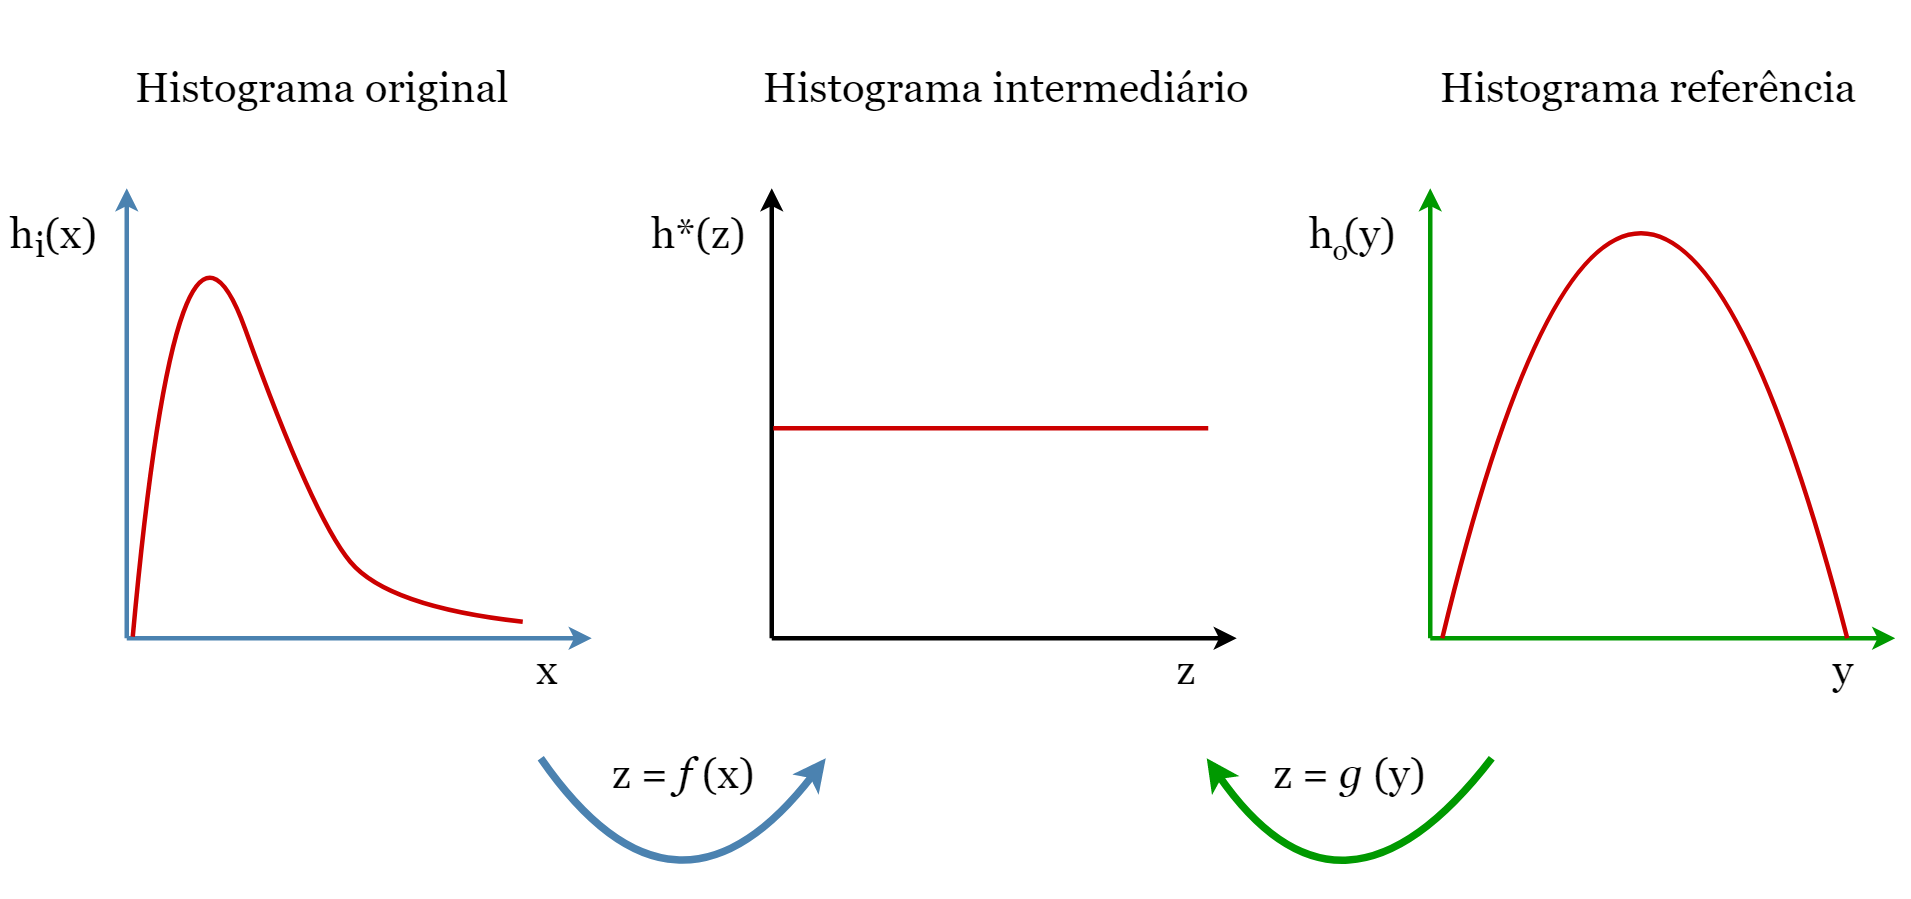
\includegraphics[width=0.9\textwidth]{figuras/especificacao-histograma.png}
%     \legend{Fonte: Adaptado de \cite{Giovanni2021}.}
%     \label{fig:especificacao_histograma}
% \end{figure}

Neste trabalho, a técnica de especificação do histograma foi usada na etapa de pré-processamento para mapear as intensidades inter-exames de TC baseado em um exame de referência de TC.

\section{Redes Neurais Artificiais}
\label{sec:redes-neurais-artificiais}

As Redes Neurais Artificiais (RNAs) são um ramo da Inteligência Artificial (IA), fundada na década de 1940, quando McCulloch e Pitts desenvolveram o primeiro modelo neural \cite{mcculloch1943logical}. O problema básico resolvido pelas RNAs é a aquisição indutiva de conceitos a partir de exemplos, a capacidade de aprender e generalizar a partir de dados, ou seja, imitar a capacidade humana de aprender com a experiência, torna as RNAs úteis na automatização do processo de aprendizado de regras de várias aplicações~\cite{MUKHOPADHYAY2011329}. 

%Em resumo, as RNAs são modelos matemáticos que usam uma coleção de unidades computacionais simples, chamadas de neurônios artificiais, interconectadas por uma grande quantidade de interconexões, denominadas sinapses artificiais~\cite{MUKHOPADHYAY2011329}. Esses modelos são comumente usados na tarefa de reconhecimento de padrões, como detecção de objetos, identificação de nódulos de câncer, reconhecimento de voz e reconhecimento facial~\cite{alanis2019artificial,baroni2020linguistic}.

Em resumo, as RNAs são esquemas computacionais que representam parcialmente as redes neurais biológicas existentes nos cérebros humanos ou animais, expressas por nós conectados (neurônios artificiais) organizados adequadamente em camadas. Todos os neurônios artificiais são conectados e capazes de transmitir sinais, geralmente números reais, por meio de suas conexões (sinapses artificiais)~\cite{MUKHOPADHYAY2011329,BERSIMIS201931}. Esses modelos são comumente usados na tarefa de reconhecimento de padrões, como detecção de objetos, identificação de nódulos de câncer, reconhecimento de voz e reconhecimento facial~\cite{alanis2019artificial,baroni2020linguistic}.

\subsection{Neurônio artificial}
\label{sec:neuronio-artificial}

O neurônio artificial é a unidade básica de uma RNA, fundamental para a construção de modelos mais poderosos. Em termos matemáticos, o neurônio artificial fornece uma saída para um determinado conjunto de entradas, conforme expresso na Equação~\ref{eq:neuronio-artificial},

\begin{equation}
\label{eq:neuronio-artificial}
f(x) = \sigma \left(\sum^n_{i=1}x_iw_i + b \right),
\end{equation}
em que $x_i$ é a entrada $i$, $w_i$ é o peso sináptico associado a entrada $i$, $b$ é o termo \textit{bias} e $\sigma$ é a função de ativação. Portanto, cada neurônio combina suas entradas e, em seguida, passa por uma função de ativação, que pode ser um filtro linear ou não-linear.

Em relação aos filtros não lineares, a função sigmoide e a função tangente hiperbólica são citadas como exemplos. Além delas, existem outra funções não lineares propostas como as chamadas~\textit{Rectified Linear Units} (ReLU) e \textit{Leaky Rectified Linear Unit} (Leaky ReLU), cuja velocidade de convergência em relação às supracitadas é até 6 vezes mais rápida~\cite{krizhevsky2012imagenet, maas2013rectifier}. Essas funções são expressas nas Equações~\ref{eq:relu} e \ref{eq:leakyrelu}, respectivamente,

\begin{equation}
\label{eq:relu}
\sigma(x) = max(0,x),
\end{equation}
\begin{equation}
\label{eq:leakyrelu}
\sigma(x) = max(0.1,x).
\end{equation}

\subsection{Redes \textit{Multilayer Percepton}}
\label{sec:redes-multilayer-percepton}

Embora existam inúmeras arquiteturas RNA, a arquitetura \textit{Multilayer Perceptron} (MLP) é a mais frequentemente encontrada na literatura \cite{PHAM2019302}. As MLPs são algoritmos de aprendizado supervisionado compostos por múltiplas camadas de neurônios, todas completamente conectadas às suas subsequentes. Os neurônios, por sua vez, implementam as funções de ativação não-linear determinadas. De acordo com \citeonline{hornik1989multilayer}, essas redes são capazes de aproximar qualquer função mensurável para qualquer grau de precisão desejado.

De modo geral, uma MLP é composta por uma camada inicial, que recebe os dados de entrada do modelo, seguida por uma ou mais camadas intermediárias (ocultas/escondidas) e, por fim, uma camada de saída~\cite{hornik1989multilayer}. A Figura~\ref{fig:rna} ilustra uma arquitetura básica de MLP com apenas uma camada oculta.

\begin{figure}[!ht]
    \centering
    \caption{Rede \textit{Multilayer Percepton}.}
    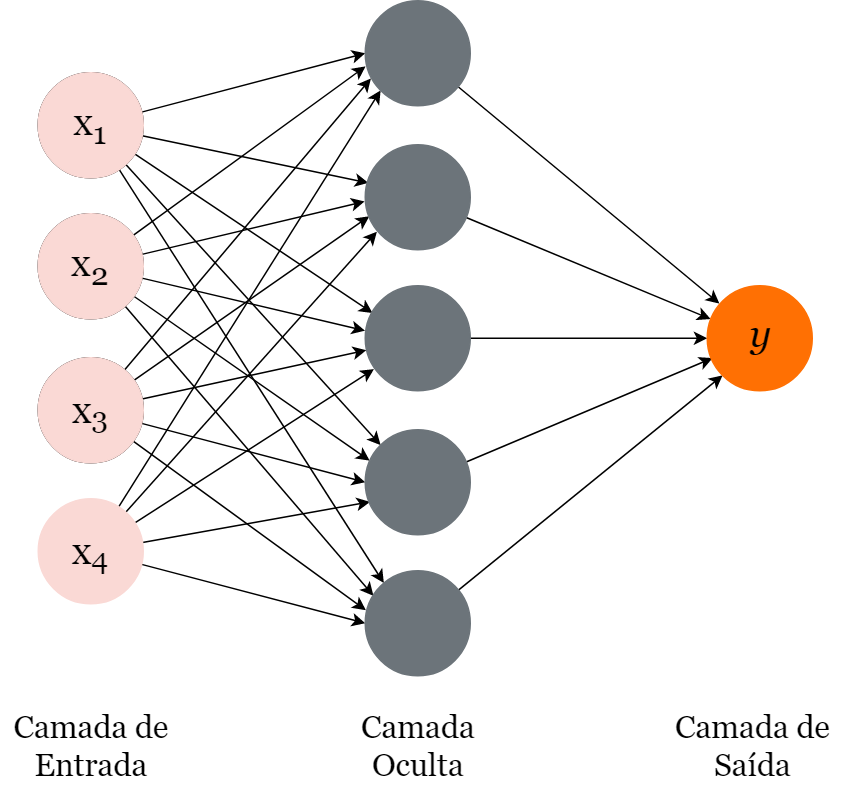
\includegraphics[width=0.45\textwidth]{figuras/RNA.png}
    \legend{Fonte: Elaborado pela autora.}
    \label{fig:rna}
\end{figure}

Os neurônios de cada camada são organizados e conectados uns aos outros em uma estrutura de múltiplas camadas \textit{feedforward}. Em outras palavras, cada camada é totalmente conectada com sua camada adjacente e produz um vetor de saída de acordo com o vetor da camada anterior~\cite{BERSIMIS201931}. A saída de cada camada é calculada aplicando a função de ativação de cada neurônio a todos os neurônios da camada. A Equação~\ref{eq:mlp} descreve a saída de uma camada,

\begin{equation}
\label{eq:mlp}
y^l = \sigma(W^ly^{l-1} + b^l),
\end{equation}
em que $y^l$ é o vetor de saída, $W^l$ é a matriz dos pesos aplicados a cada par de neurônio da camada $l$ e $l-1$, e $b^l$ é o vetor do termo \textit{bias} de cada neurônio da camada $l$. Para treinar efetivamente as MLPs, o algoritmo de \textit{backpropagation} é aplicado.

\subsection{\textit{Backpropagation}}
\label{sec:backpropagation}

Durante o treinamento de uma MLP, uma função de erro é definida para calcular o erro das predições do modelo com base na saída esperada para os dados de entrada fornecidos. O objetivo do treinamento é minimizar o erro total da rede (soma das funções de erro aplicadas a todos os exemplos de uma base de imagens). Para isso, as MLPs usam um algoritmo denominado \textit{backpropagation}.

O algoritmo \textit{backpropagation} é caracterizado por dois passos consecutivos: primeiro, os dados são enviados para a camada de entrada da rede, e trafegam pela rede, camada por camada, sendo transformados por meio de cálculos realizados até que, na camada de saída, uma resposta seja produzida; segundo, a saída obtida é comparada com a saída desejada da entrada correspondente e um valor de erro é calculado. Em seguida, os erros derivados com relação aos parâmetros da rede são propagados novamente, da camada de saída até a camada de entrada, desta forma, os pesos das conexões nas camadas ocultas são modificados à medida que o erro é retropropagado. O processo continua várias vezes até que uma melhoria desejada na previsão do modelo seja alcançada.

Os passos do algoritmo~\textit{backpropagation} são brevemente apresentados a seguir. Os itens 1, 2 e 3 estão relacionados ao \textit{feedforward} e o \textit{backpropagation} inicia no item 4.

\begin{enumerate}
	\item Inicializar os valores dos pesos sinápticos de cada neurônio aleatoriamente;
	
	\item Apresentar as entradas da rede em um vetor ${x_1 , x_2 , ..., x_n}$ de características e especificar um vetor ${d_1 , d_2 , ..., d_n}$ de saídas desejadas;
	
	\item Calcular as saídas da rede ${y_1 , y_2 , ..., y_n}$ conforme a Equação~\ref{eq:neuronio-artificial};
	
	\item Reajustar os pesos começando pelos neurônio da camada de saída, retropropagando até a camada de entrada, de acordo com a Equação~\ref{eq:bp1},
    \begin{equation} \label{eq:bp1}
    	w_{ij} (t + 1)= w_{ij} (t) + \eta \delta_j x_i,
    \end{equation}
	onde $w_{ij}$ é o peso do neurônio $j$ em uma iteração $t$, $x_i$ corresponde a um neurônio de saída ou de entrada, $\eta$ é a taxa de aprendizagem e $\delta_j$ é um erro de gradiente para o neurônio $j$. Se $j$ for um neurônio de saída, então $\delta_j$ é definido pela Equação~\ref{eq:bp2},
	\begin{equation}
	\label{eq:bp2}
    	\delta_j = y_j (1 - y_j)(d_j - y_j),
    \end{equation}
	onde $d_j$ denota a saída desejada e $y_j$ é a saída desejada da rede. Se o neurônio $j$ for um neurônio oculto, então $\delta_j$ é definido pela Equação~\ref{eq:bp3},
	\begin{equation}
	\label{eq:bp3}
        \delta_j = x_j (1 - x_j) \sum_{k}\delta_k w_{jk},
    \end{equation}
	onde $k$ denota todos os neurônios da camada após a camada do neurônio $j$;
	\item Retornar ao passo 2 até que uma determinada condição seja satisfeita.
\end{enumerate}

É importante ressaltar que a taxa de aprendizado ($\eta$) influencia a magnitude das mudanças dos pesos, desempenhando papel fundamental no aprendizado do modelo. Taxas de aprendizados muito pequenas implicam em pequenas variações, o que torna o modelo lento e aumentam as chances de parar em mínimos locais. No entanto, altas taxas de aprendizado tendem a produzir grandes oscilações, o que compromete o processo de aprendizado do modelo. A taxa de aprendizado é introduzida na rede para permitir uma convergência mais rápida ao valor ótimo desejado e ao mesmo tempo evitar que a rede oscile, diminuindo a taxa de aprendizado quando o erro tende a aumentar~\cite{silva2004algoritmos,haykin2007redes,silva2010redes}.

%Uma vez que a rede está treinada e o erro está em um nível satisfatório, a rede pode ser usada como uma ferramenta para classificar novos dados.

\section{Aprendizado Profundo}
\label{sec:aprendizado-profundo}

Durante o processo de aprendizagem, humanos e animais são inicialmente conduzidos a interpretar e compreender conceitos mais simples, a fim de aprender conceitos mais complexos a partir de conceitos previamente observados ao longo de suas vidas~\cite{fernandes2013redes}. Esse processo de aprendizagem, denominado aprendizado profundo, sugere uma divisão em camadas hierárquicas do cérebro com diferentes responsabilidades~\cite{hubel1998early}.

O aprendizado profundo é uma subárea do aprendizado de máquina que usa arquiteturas hierárquicas para aprender abstrações de alto nível em um conjunto de imagens. É uma abordagem em evolução e tem sido amplamente usada em domínios tradicionais de inteligência artificial, como análise semântica, transferência de aprendizado, processamento de linguagem natural e visão computacional. Existem três fatores importantes para o crescimento do aprendizado profundo: o aumento da capacidade de processamento dos \textit{chips} gráficos, os avanços consideráveis nos algoritmos de aprendizado de máquina e o custo significativamente reduzido do \textit{hardware} de computação~\cite{GUO201627}.

As técnicas de aprendizagem profunda apresentam múltiplas camadas de processamento não linear para reconhecimento de padrões de forma semelhante ao cérebro~\cite{LeCun2015}. Diferente das RNAs tradicionais, essas técnicas permitem a extração automática de características do conjunto de treinamento, sem a necessidade de uma série de técnicas de processamento de imagens e reconhecimento de padrões~\cite{hua2015computer}. Como resultado, as etapas de extração, seleção e classificação de características são abstraídas no próprio modelo, com pouca intervenção humana~\cite{hua2015computer,cheng2016computer}.

Atualmente, existem inúmeras técnicas de aprendizagem profundas disponíveis na literatura, como as redes neurais convolucionais, redes neurais recorrentes, redes de crença profunda, redes de memória de longo prazo, os auto-codificadores esparsos empilhados, entre outras. As diferentes arquiteturas têm diferentes vantagens com base na aplicação e nas características dos dados envolvidos. Por exemplo, em visão computacional, as redes neurais convolucionais são preferidas e, em sequências e modelagem de séries temporais, as redes neurais recorrentes. O aprendizado profundo é um campo em rápida evolução e arquiteturas mais novas com algoritmos de aprendizado mais recentes são frequentemente desenvolvidas para suportar a necessidade de desenvolver máquinas eficientes semelhantes a humanos em diferentes áreas de aplicação~\cite{SENGUPTA2020}.

\subsection{Redes Neurais Convolucionais}
\label{sec:redes-neurais-convolucionais}

As redes neurais convolucionais (\textit{Convolutional Neural Networks} - CNN) são modelos biologicamente inspirados capazes de construir um aprendizado hierárquico de características~\cite{726791, 6932467}. Essa arquitetura é bastante popular em tarefas de visão computacional, como detecção, segmentação e classificação de imagens e vídeos de vários domínios.

Geralmente, a CNN usa em sua arquitetura três tipos de camadas: convolução, subamostragem e completamente conectada~\cite{726791}. As camadas de convolução extraem características de baixo nível importantes da imagem de entrada, como textura simples e bordas. À medida que mais camadas de convolução são adicionadas, características de alto nível são extraídas. As camadas de subamostragem reduzem a resolução dos mapas de características, mantendo as informações de características. Finalmente, a camada totalmente conectada conecta a rede à camada discriminante (camada de saída), que fornece a saída desejada~\cite{LeCun2015}. A Figura~\ref{fig:cnn} ilustra uma arquitetura básica de CNN, em seguida, os detalhes de cada camada são apresentados.

\begin{figure}[!ht]
    \centering
    \caption{Exemplo de uma arquitetura CNN.}
    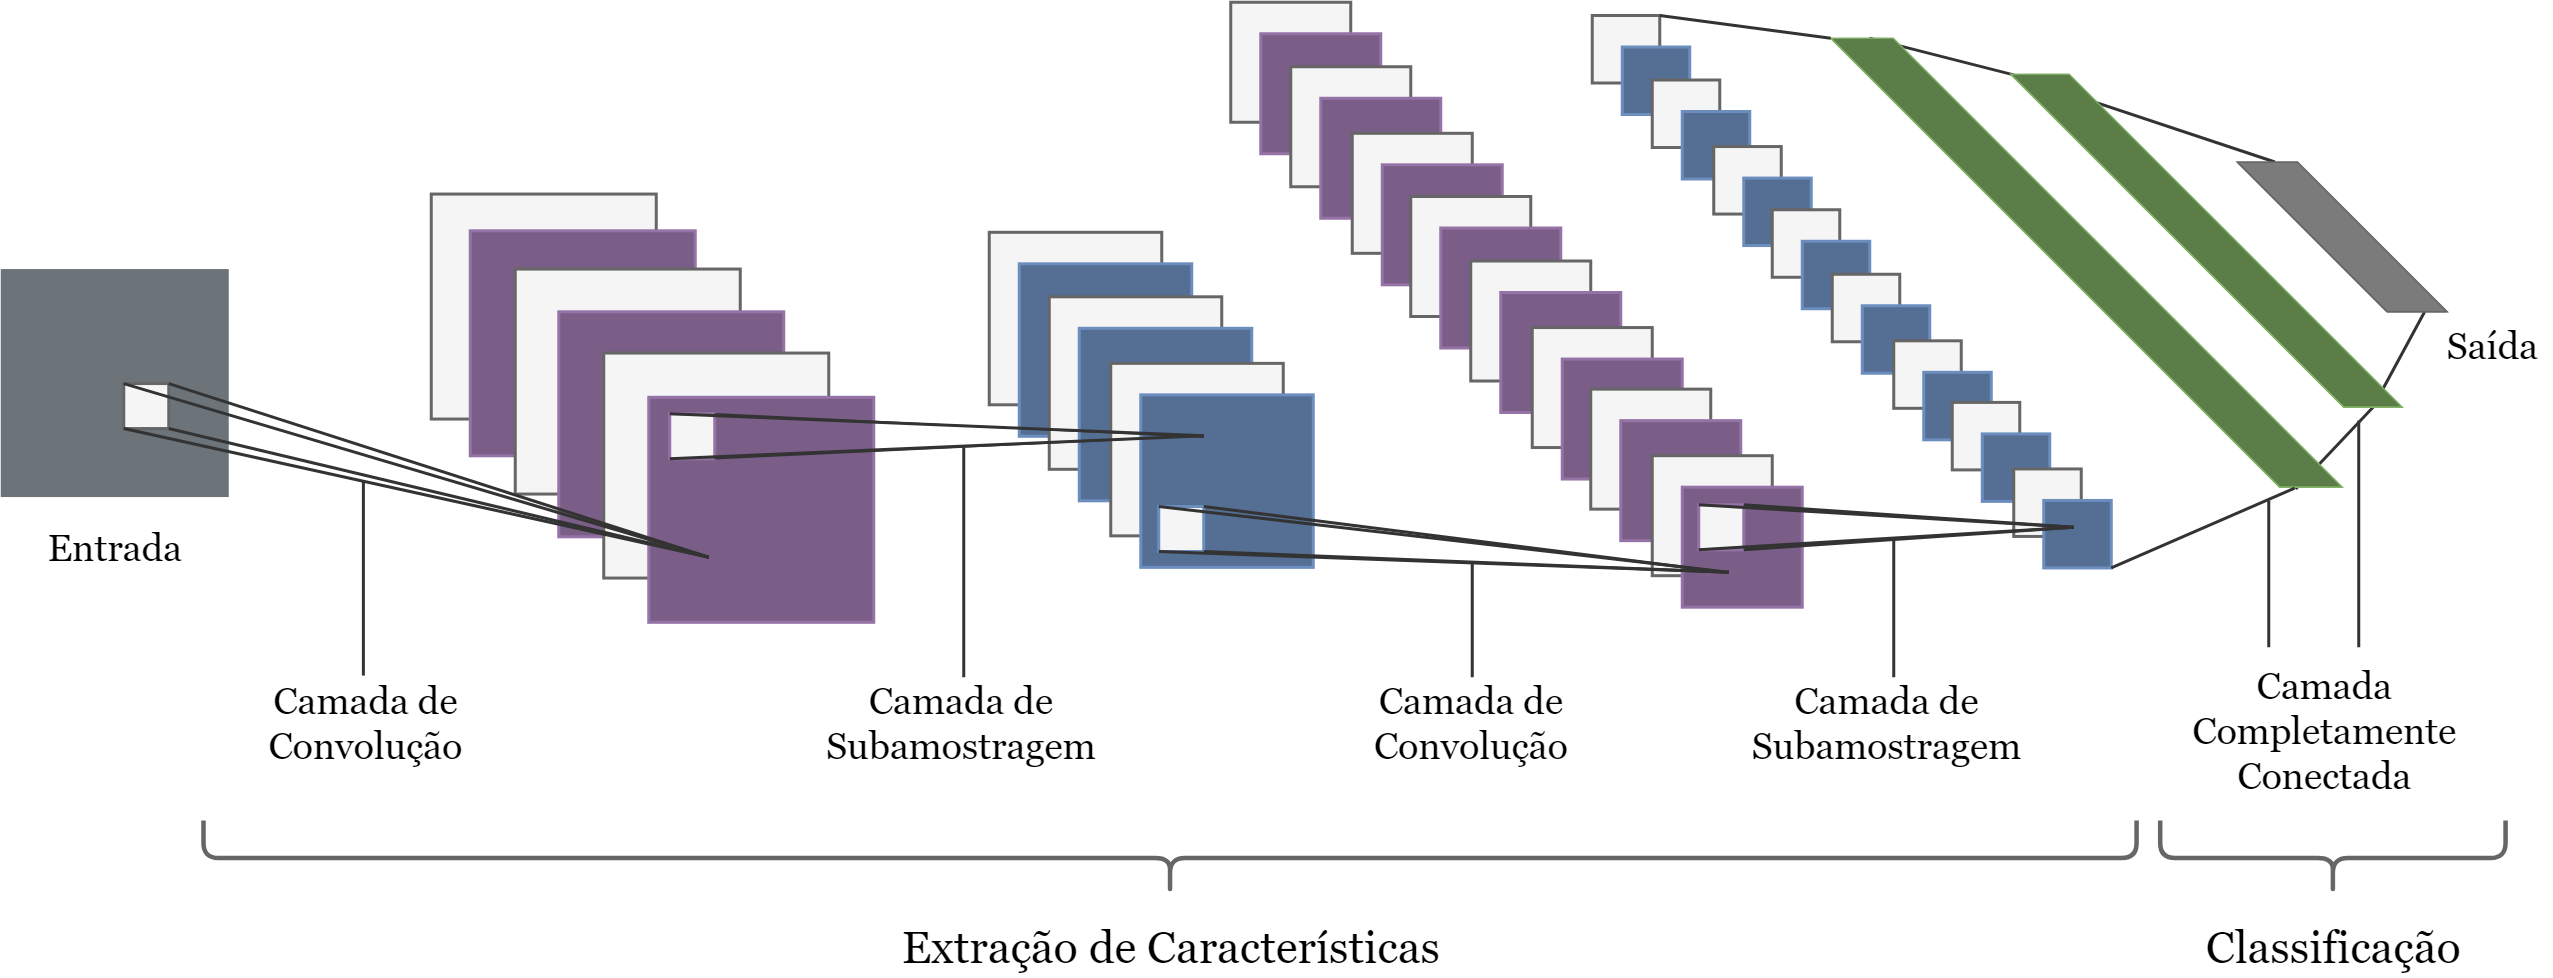
\includegraphics[width=1\textwidth]{figuras/arquitetura-CNN.png}
    \legend{Fonte: Adaptado de \cite{LIU201711}.}
    \label{fig:cnn}
\end{figure}

\subsubsection{Camada de Convolução}
\label{sec:camada-convolucao}

As camadas de convolução são compostas por filtros treináveis aplicados individualmente na imagem de entrada da rede, gerando diversos mapas de características. Os filtros são definidos por uma pequena área ($3\times3$, $5\times5$, $7\times7$ \textit{pixels}) e cada neurônio é ligado apenas aos neurônios nas proximidades da camada anterior. Portanto, para cada filtro aplicado a uma imagem de entrada, pode existir um neurônio conectado com a saída de um subconjunto de neurônios da camada anterior. Os pesos são compartilhados entre os neurônios, fazendo com que os filtros aprendam os padrões frequentes que ocorrem em qualquer parte da imagem~\cite{5537907,GUO201627}. O processo de convolução em uma imagem é ilustrado na Figura~\ref{fig:camada-convolucao}.

\begin{figure}[!ht]
    \centering
    \caption{Ilustração de uma operação de convolução.}
    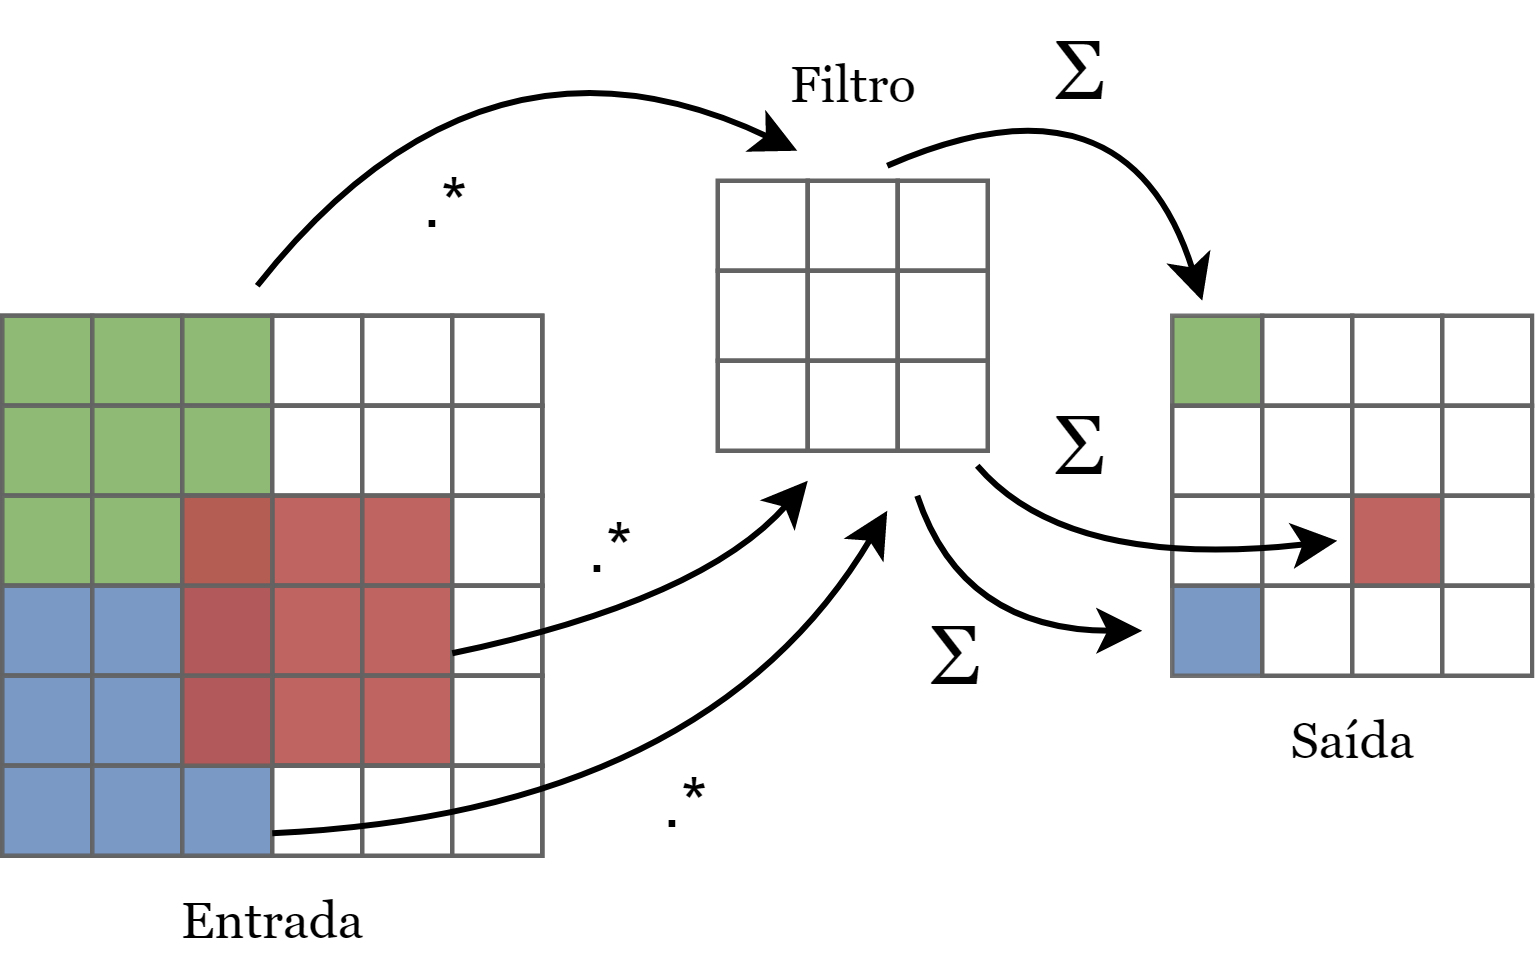
\includegraphics[width=0.57\textwidth]{figuras/camada-convolucao.png}
    \legend{Fonte: Adaptado de \cite{hafemann:14}.}
    \label{fig:camada-convolucao}
\end{figure}

Após gerar mapas de características, uma camada de ativação não linear é aplicada~\cite{WU2020}. Ao fim do treinamento da rede, cada filtro será responsável por detectar uma característica específica da imagem, ou de parte dela~\cite{hafemann:14}.

\subsubsection{Camada de Subamostragem}
\label{sec:camada-subamostragem}

As camadas de subamostragem são geralmente subsequentes às camadas de convolução e são usadas para reduzir as resoluções dos mapas de características produzidos pelas camadas de convoluções anteriores e selecionar as características invariantes a deslocamentos e distorções~\cite{5537907,hafemann:14}.

A subamostragem consiste em aplicar filtros nos mapas de características e usar operações como média (\textit{average pooling}) ou valor máximo (\textit{max-pooling}) para extrair valores dessas sub-regiões. A Figura~\ref{fig:camada-subamostragem} ilustra a subamostragem com a aplicação da operação \textit{max-pooling} deslizando uma janela de tamanho 3 com passo igual a 1, na qual apenas o valor máximo de \textit{pixel} da janela de convolução é mantido. Ou seja, em uma máscara $3\times3$ com 9 valores, apenas o maior valor de \textit{pixel} entre eles permanecerá.

\begin{figure}[!ht]
    \centering
    \caption{Ilustração da camada de subamostragem.}
    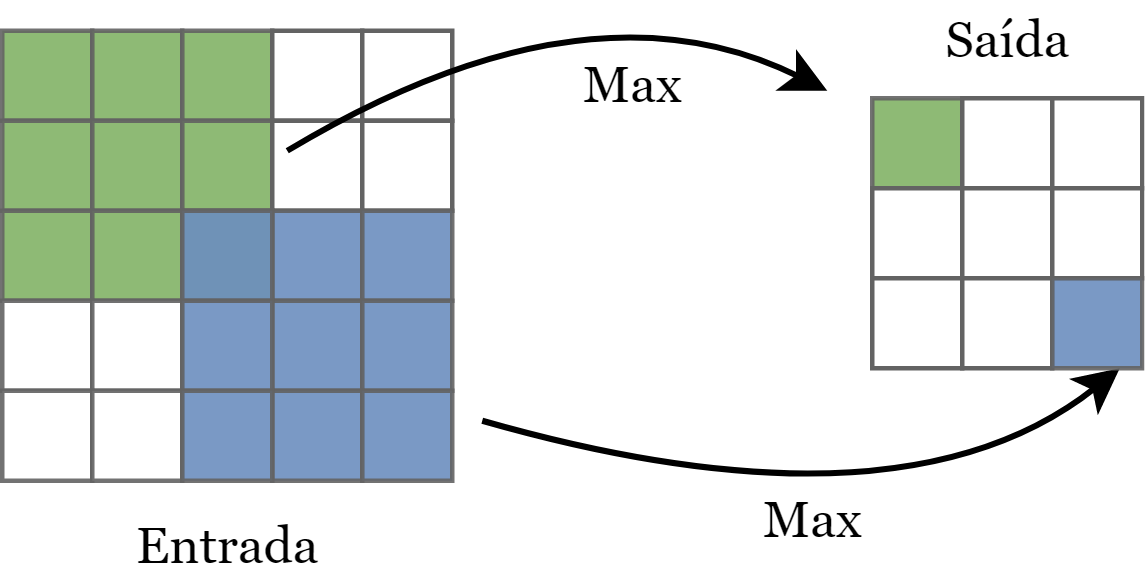
\includegraphics[width=0.55\textwidth]{figuras/camada-subamostragem2.png}
    \legend{Fonte: Adaptado de \cite{hafemann:14}.}
    \label{fig:camada-subamostragem}
\end{figure}

Existem também as operações de \textit{upsampling}. Basicamente, elas se comportam como o inverso das camadas de~\textit{max-pooling}, ou seja, dobram a resolução dos mapas de características da camada anterior por operações de interpolação~\cite{long2015fully}. No entanto, é configurável.

\subsubsection{Camada Completamente Conectada}
\label{sec:camada-completamente-conectada}

Depois de extrair as características com as camadas de convolução e subamostragem, os mapas de características podem ser usados como entrada para as camadas totalmente conectadas, que por sua vez são responsáveis por classificar os padrões de entrada. Os neurônios em uma camada totalmente conectada têm conexões com todas as ativações na camada anterior, semelhante à estrutura do MLP (Seção~\ref{sec:redes-multilayer-percepton}).

Uma vez que a rede esteja treinada em um nível satisfatório, a rede pode ser usada como uma ferramenta para classificar novos dados. Neste trabalho, arquiteturas baseadas nos conceitos de redes neurais convolucionais são usadas para segmentar rins e tumores renais em imagens tomográficas.

\section{Arquitetura U-Net}
\label{sec:arquitetura-unet}

Para realizar a segmentação dos rins e reconstrução dos tumores renais em imagens de TC, foi usada como base a arquitetura da U-Net~\cite{He7780459}, que é uma rede capaz de generalizar mesmo em domínio de baixa variância.

A U-Net é uma RNA completamente convolucional proposta para segmentação de imagens biomédicas \cite{ronneberger2015u}, que desde 2015 vem superando os métodos existentes em diversos desafios biomédicos de segmentação de imagens. Essa rede é um tipo específico de rede profunda e avançada cuja arquitetura consiste em um caminho de contração e um caminho de expansão simétrico. A principal estratégia que diferencia a U-Net das outras arquiteturas totalmente convolucionais (\textit{Fully Convolutional Network} - FCN) é a combinação entre os mapas de características no estágio de contração e seus correspondentes simétricos no estágio de expansão, o que permite a propagação de informações de contexto para os mapas de características de alta resolução. A Figura~\ref{fig:arquitetura_unet} ilustra a arquitetura e as camadas que constituem a U-Net.

\begin{figure}[!ht]
    \centering
    \caption{Arquitetura U-Net.}
    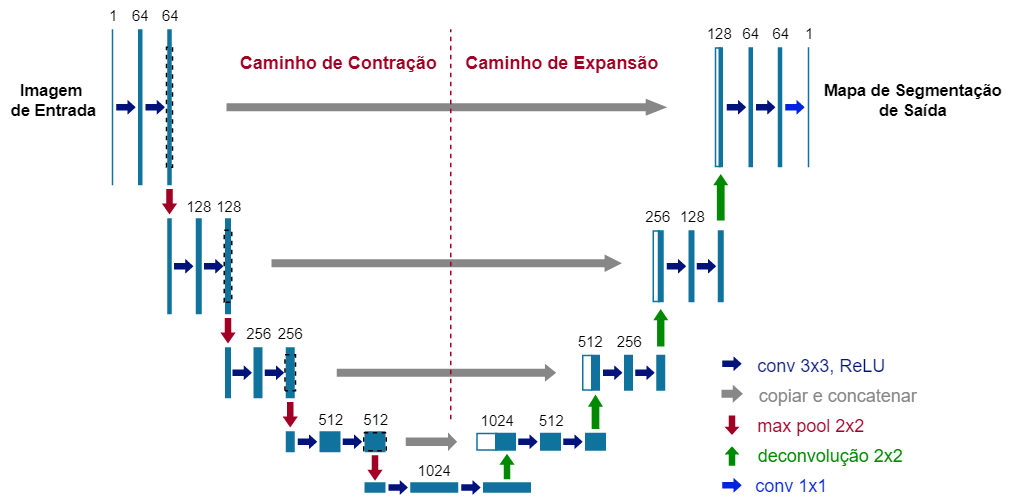
\includegraphics[width=1\textwidth]{figuras/arquitetura-Unet.png}
    \legend{Fonte: Adaptado de \cite{ronneberger2015u}.}
    \label{fig:arquitetura_unet}
\end{figure}

O caminho de contração (lado esquerdo) captura o contexto e o caminho de expansão (lado direito) simétrico permite uma localização precisa. O caminho de contração é uma arquitetura CNN tradicional, várias aplicações repetidas de duas convoluções $3\times3$, cada uma acompanhada por uma função de ativação ReLU e uma operação de subamostragem com operação de \textit{max-pooling} $2\times2$, reduzindo a largura e a altura da imagem, com passo (\textit{stride}) 2 para subamostragem. Em cada etapa de subamostragem, o número de canais de características dobra.  No caminho de contração as camadas de 1 a 5 são compostas por convoluções de 64, 128, 256, 512 e 1024 filtros, respectivamente.

O caminho de expansão consiste em um levantamento do mapa de características seguido de uma deconvolução (\textit{upsampling}) $2\times2$ que faz a metade do número de canais de características. Posteriormente, uma junção é feita com o mapa de características correspondentemente cortado do caminho de contratação e duas convoluções 3x3, cada uma seguida por uma função de ativação ReLU. Essa etapa do caminho expansivo é importante devido à perda de \textit{pixels} de borda em cada convolução no caminho de contratação. Na última camada é usada uma convolução 1x1 para mapear cada vetor de características para o número desejado de classes.

Em resumo, a U-Net pode ser treinada do início ao fim com poucas imagens, onde a U-Net simplesmente concatena os mapas de características do codificador para mapear mapas de características do decodificador em todas as etapas para formar uma estrutura como escada. As conexões de concatenação nesta arquitetura permitem que o decodificador aprenda as características relevantes que são perdidas quando o codificador é agrupado em cada fase.

\section{Arquitetura DeepLabv3+}
\label{sec:deeplabv3+}

Para obter a segmentação de tumores renais em TC, foi usada como base a arquitetura de última geração DeepLabv3+~\cite{chen2018encoder}, que é um modelo forte para codificar informações contextuais e refinar os resultados da segmentação, especialmente ao longo dos limites do objeto.

Como descrito anteriormente, as redes neurais profundas usam estruturas de codificador-decodificador para tarefas de segmentação semântica. O codificador extrai informações contextuais em várias escalas, enquanto o decodificador captura os limites dos objetos de forma mais clara, recuperando gradualmente as informações espaciais para reconstruir a saída~\cite{chen2018encoder}. Na arquitetura DeepLabv3+ o codificador padrão usado é o Xception (\textit{Extreme Inception})~\cite{chollet2017xception}. Em resumo, o Xception é uma extensão da arquitetura Inception que substitui os módulos Inception padrão por convoluções separáveis em profundidade (\textit{depth wise separable convolution}).

A Figura~\ref{fig:arquitetura_DeepLabv3+} ilustra a arquitetura DeepLabv3+. As imagens de entrada da rede passam por uma estrutura de codificador-decodificador. Na fase de codificação, as características extraídas do codificador Xception são usadas como entrada para as operações de \textit{Atrous Convolution} e \textit{Atrous Spatial Pyramid Pooling} (ASPP). O \textit{Atrous Convolution} captura características em escalas múltiplas (\textit{rate} = 6, \textit{rate} = 12 e \textit{rate} = 18), e o ASPP é uma operação de \textit{pooling} que ajuda a calcular objetos em escalas diferentes. Essas operações fazem a ponte entre a codificação e a decodificação~\cite{chen2018encoder}.

\begin{figure}[!ht]
    \centering
    \caption{Arquitetura DeepLabv3+.}
    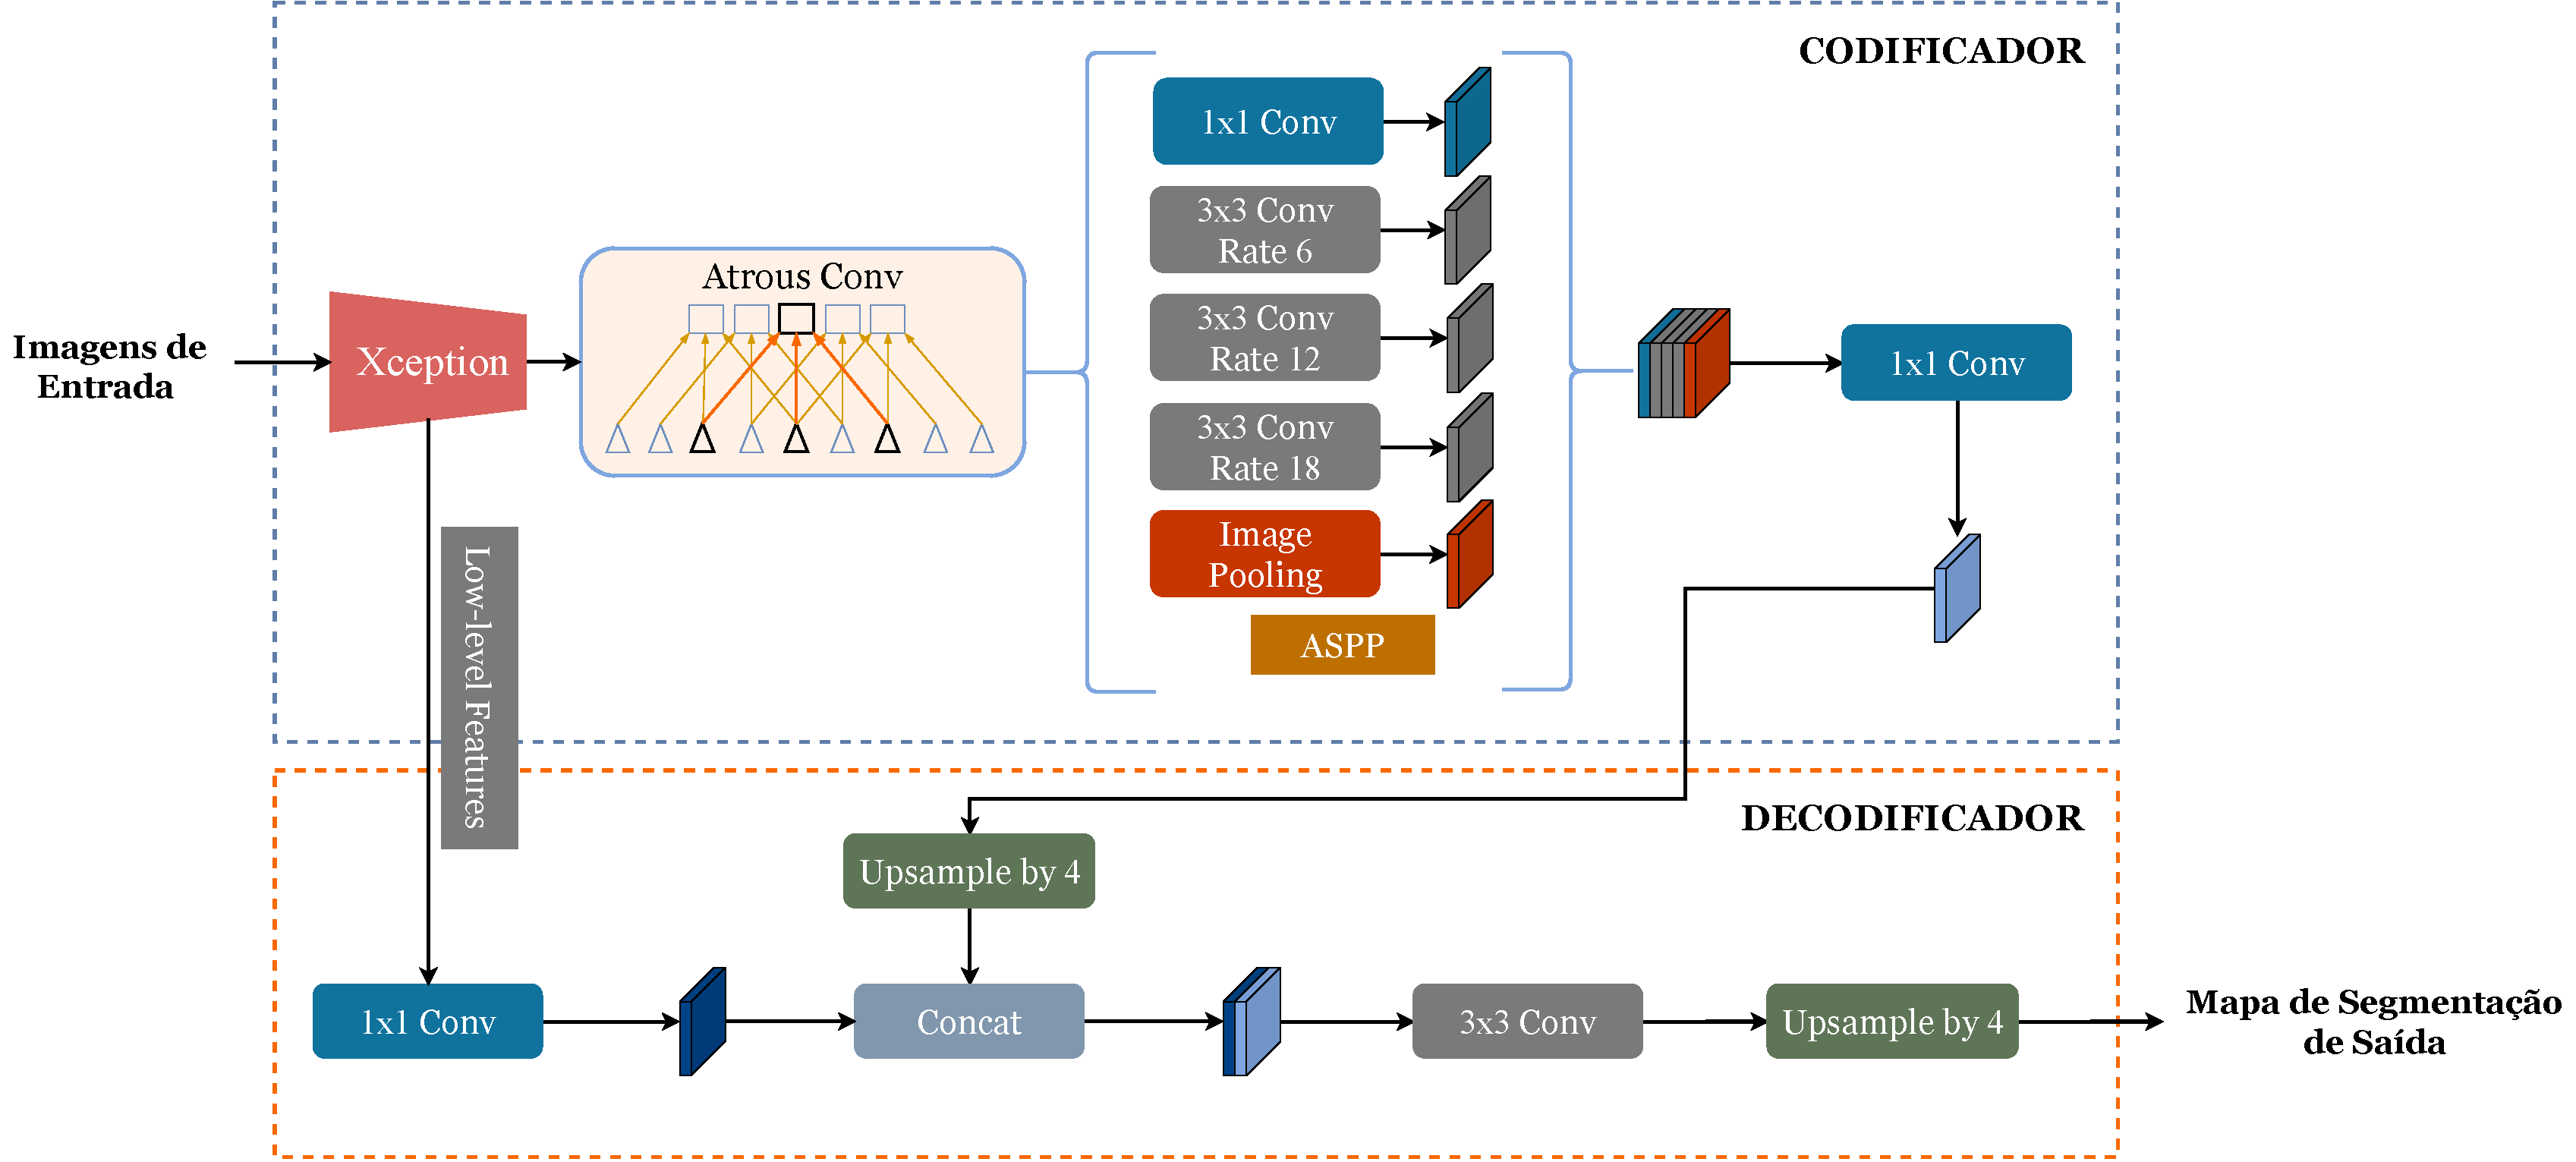
\includegraphics[width=1\textwidth]{figuras/arquitetura_DeepLabv3+.pdf}
    \legend{Fonte: Adaptado de~\cite{chen2018encoder}.}
    \label{fig:arquitetura_DeepLabv3+}
\end{figure}

Na fase de decodificação, as informações extraídas na codificação são usadas para reconstruir a saída. Assim, após as operações de \textit{Atrous Convolution} e ASPP, a operação de \textit{upsampling} é aplicada usando um filtro bilinear de fator 4. Posteriormente, concatena-se com os \textit{low-level features} (características de baixo nível) correspondentes da saída do codificador Xception, após passar por uma convolução 1 × 1 para reduzir o número de canais. Após a concatenação, algumas convoluções 3 × 3 são aplicadas para refinar as características, seguidas por outro \textit{upsampling} bilinear simples de fator 4. Além disso, é usada a \textit{depth wise separable convolution}, que é uma operação para reduzir o custo de computação e vários parâmetros, mantendo o desempenho~\cite{chen2018encoder}.

\section{\textit{Data Augmentation}}
\label{sec:data-augmentation}

\textit{Data augmentation} é uma técnica comumente usada na literatura para aumentar o tamanho e a diversidade dos conjuntos de treinamento. Em visão computacional, o \textit{data augmentation} se tornou uma técnica de regularização implícita comum para combater o \textit{overfitting} em modelos de aprendizado profundo e é usado para melhorar o desempenho do modelo~\cite{kukavcka2017regularization, mikolajczyk2018data}.

O aumento de dados é semelhante à imaginação ou sonho. Os seres humanos imaginam diferentes cenários com base na experiência. A imaginação ajuda a compreender melhor o mundo. Os métodos de \textit{data augmentation}, podem “imaginar” alterações nas imagens, para que tenham um melhor entendimento delas~\cite{shorten2019survey}. Portanto, técnicas são usadas para aumentar a diversidade da base de imagens aplicando transformações aleatórias, como transformações geométricas (rotação, translação, espelhamento, etc.) e filtros para realçar imagens (CLAHE, filtros de contraste, etc.), por exemplo.

No entanto, existem algumas desvantagens de usar o \textit{data augmentation}, como memória e tempo de treinamento adicionais, e alto custo computacional~\cite{shorten2019survey}. Estas desvantagens ocorrem quando o \textit{data augmentation} é gerado \textit{offline} (em disco) e adicionado ao conjunto de treinamento. Como não é prático nem eficiente armazenar os dados aumentados na memória, técnicas de \textit{data augmentation} em tempo real são usadas como uma solução para minimizar essas desvantagens. Como o nome sugere, o aumento é aplicado em tempo real, as transformações são realizadas em mini-lotes e, em seguida, inseridas ao treinamento do modelo. Dessa forma, as variações criadas artificialmente a partir de imagens existentes não precisam ser salvas na memória do disco, o que reduz o tempo de acesso ao disco para realizar operações de leitura e escrita.

No método proposto, o \textit{data augmentation} foi realizado em tempo real (\textit{online})~\cite{shorten2019survey}, não sendo necessário incluir novas imagens de \textit{data augmentation} no conjunto de treinamento original, uma vez que foi aplicado diretamente ao conjunto de treinamento. Desta forma, novas imagens são geradas atualizando constantemente o próprio conjunto de treinamento. Essa técnica proporcionou maior poder de generalização e desempenho do modelo e baixo consumo de recursos de máquina. Na subseção~\ref{sec:resultados-candidatores-tumores-renais-regiao-renal} são apresentadas as operações de \textit{data augmentation} em tempo real que foram aplicadas neste estudo.

\section{Métricas de Desempenho}
\label{sec:metricas-de-desempenho}

Para validar os resultados obtidos por um método proposto, quantificações de resultados são comumente adotadas. Esta atividade tem como objetivo avaliar o desempenho do método desenvolvido por meio da análise estatística dos resultados. Neste trabalho, as métricas usadas são comumente aplicadas em sistemas CAD/CADx para análise de imagens médicas: acurácia, sensibilidade, especificidade, coeficiente de similaridade Dice e índice de Jaccard~\cite{taha2015metrics, bland2015introduction}.

%Para o cálculo das métricas, baseou-se na matriz de confusão (Figura~\ref{fig:matriz_confusao}), que leva em consideração 4 variáveis: (1) Verdadeiro Positivo (VP) indica os casos realmente positivos detectados; (2) Falso Positivo (FP) denota os casos negativos erroneamente detectados como positivos; (3) Verdadeiro Negativo (VN) denota os casos negativos verdadeiramente detectados; e (4) Falso Negativo (FN) denota os casos positivos detectados erroneamente como negativos.

O cálculo das métricas é baseado na matriz de confusão (Figura~\ref{fig:matriz_confusao}), que leva em consideração quatro variáveis: Verdadeiro Positivo (VP) indica a classificação correta dos \textit{pixels} da classe positiva, ou seja, o alvo de segmentação (rins ou tumores renais, dependendo do modelo); Falso Positivo (FP) denota a classificação errônea dos \textit{pixels} da classe negativa como classe positiva; Verdadeiro Negativo (VN) indica a classificação correta dos \textit{pixels} da classe negativa; e Falso Negativo (FN) trata-se da classificação errônea dos \textit{pixels} da classe positiva como classe negativa.

\begin{figure}[!ht]
    \centering
    \caption{Matriz de confusão.}
    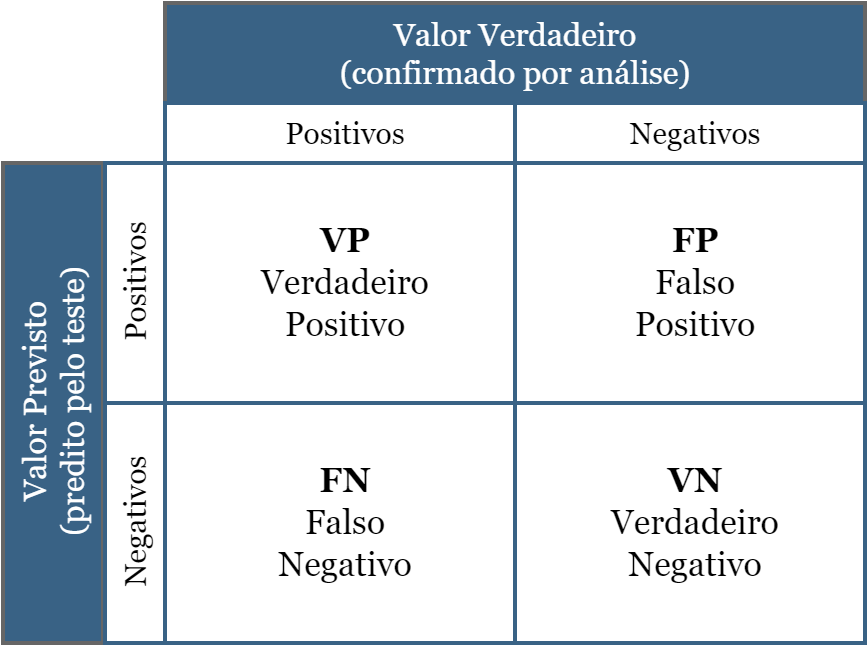
\includegraphics[width=0.4\textwidth]{figuras/matriz_confusao2.png}
    \legend{Fonte: Adaptado de \cite{diniz2021metodos}.}
    \label{fig:matriz_confusao}
\end{figure}

A acurácia (Acc) é definida como a razão entre o número de \textit{pixels} classificados corretamente (classe positiva e negativa) e o número total de \textit{pixels} na amostra do estudo. O cálculo da acurácia é expressa na Equação \ref{eq:acuracia},

\begin{equation}
\label{eq:acuracia}
Acc = \frac{VP + VN}{VP + VN + FP + FN}.
\end{equation}

A sensibilidade (Sen) é a capacidade do sistema em predizer corretamente a classe positiva, ou seja, indica a proporção de verdadeiros positivos. O cálculo da sensibilidade é definida na Equação \ref{eq:sensibilidade},

\begin{equation}
\label{eq:sensibilidade}
Sen = \frac{VP}{VP + FN}.
\end{equation}

A especificidade (Esp) é a capacidade do sistema em predizer corretamente a classe negativa, ou seja, a proporção de verdadeiros negativos. O cálculo da especificidade é definido na Equação \ref{eq:especificidade},

\begin{equation}
\label{eq:especificidade}
Spe = \frac{VN}{VN + FP}.
\end{equation}

O Dice, também conhecido como F-score e F-measure, é mais usada na validação da segmentação de imagens médicas \cite{taha2015metrics}. É uma estatística usada para comparar a similaridade de duas amostras. Neste trabalho, é usado para comparar a marcação do especialista e a marcação produzida pelo método. A Equação~\ref{eq:dice} define o cálculo do Dice,

\begin{equation}
\label{eq:dice}
Dice = \frac{2VP}{2VP + FP + FN}.
\end{equation}

O índice de Jaccard (Jacc), também conhecido como \textit{Intersection over Union} (IoU), busca apresentar de forma objetiva o nível de similaridade entre duas amostras. Pode ser calculado pela razão entre a intersecção de dois conjuntos (marcação obtida pelo método e marcação do especialista) e sua união. Em matrizes de confusão empregadas para classificação binária, o índice de Jaccard pode ser descrito pela Equação~\ref{eq:jaccard},

\begin{equation}
\label{eq:jaccard}
Jacc = \frac{VP}{VP+FP+FN}.
\end{equation}

Além disso, foi realizado o teste de significância que é um procedimento estatístico que permite tomar uma decisão entre duas ou mais hipóteses (rejeitar ou não rejeitar), usando os dados observados de um determinado experimento~\cite{statistical1982, zou2003}. Assim, usamos o teste de significância entre os resultados das abordagens apresentados no Capítulo~\ref{cap:resultados}. Para isso, é necessário encontrar o \textit{p-value}, que é uma espécie de teste de significância. Inicialmente, devem ser especificados os elementos para a formulação de um plano de análise, são eles: o método de teste e o nível de significância. O método de teste usado foi o teste z de duas proporções~\cite{zou2003}, pois determina a diferença hipotética entre duas abordagens. O teste z é apropriado quando o tamanho da amostra é relativamente grande e possui uma distribuição normal. E o nível de significância adotado foi $\alpha$ = 0,05, onde $p>0,05$ não rejeita a hipótese nula, o que indica que não há diferença significativa entre as abordagens. O nível de significância aplicado é o mais frequentemente adotado na literatura~\cite{gauvreau19945}.

Todas as métricas descritas visam mensurar o desempenho do método proposto como satisfatório ou não, bem como evidenciar aspectos positivos e negativos para trabalhos futuros.

\section{Considerações Finais}

Neste capítulo, foi apresentada a fundamentação teórica necessária para a compreensão das técnicas utilizadas e suas aplicações no método proposto. Foram abordados temas como: rins e tumores renais, exame de TC, técnicas de pré-processamento digital de imagens, aprendizado profundo e métricas de desempenhos.